\documentclass[11pt,a4paper]{article}

\usepackage[utf8]{inputenc}
\usepackage[T1]{fontenc}
\usepackage{amsmath,amssymb,amsfonts}
\usepackage{graphicx}
\usepackage{booktabs}
\usepackage{siunitx}
\usepackage{geometry}
\usepackage{hyperref}
\usepackage{caption}
\usepackage{subcaption}
\usepackage{listings}
\usepackage{xcolor}
\usepackage{float}

\geometry{margin=2.5cm}

\title{Thesis Progress Report: Porto Dataset Conversion Tool}
\author{Guy Tordjman}
\date{\today}

\begin{document}

\maketitle

\tableofcontents
\newpage

\section{Introduction}

This document summarizes the progress made on the thesis work over the past month, focusing on the development of a tool to convert Porto taxi trajectory data into DSTRA dataset format and sensor-based datasets. The tool is currently in a partially completed state, with several challenges identified that need to be addressed.

\section{Why Not Use Simulation-Only Datasets?}

While simulation-based datasets (such as those generated with SUMO) offer several advantages including complete control over traffic scenarios, ground-truth route information, and dynamic graph structures, they have significant limitations for real-world ETA prediction:

\begin{itemize}
    \item \textbf{Lack of Real-World Complexity}: Simulated traffic patterns may not capture the full complexity of real-world driving behaviors, including unpredictable driver decisions, emergency situations, and non-standard traffic patterns.
    \item \textbf{Validation Concerns}: Models trained exclusively on simulated data may not generalize well to real-world scenarios, as they may learn patterns specific to the simulation rather than actual traffic dynamics.
    \item \textbf{Data Distribution Mismatch}: The distribution of travel times, speeds, and congestion patterns in simulation may differ substantially from real-world distributions, leading to poor model performance when deployed.
    \item \textbf{Missing Real-World Features}: Real-world datasets contain noise, GPS inaccuracies, and other artifacts that models must be robust to. Training only on clean simulated data may result in models that fail in production environments.
\end{itemize}

Therefore, while simulation datasets are valuable for initial model development and controlled experiments, it is essential to validate and enhance models using real-world data to ensure practical applicability.

\section{Existing ETA Prediction Datasets and Their Characteristics}

\subsection{Flow Prediction Datasets}

Traditional traffic flow prediction datasets such as METR-LA, PeMS-Bay, and SEATTLE Loop provide aggregated sensor readings but lack individual vehicle trajectories and explicit route information. These datasets are suitable for flow forecasting but not for ETA prediction at the vehicle level.

\subsection{Trip-Based ETA Datasets}

Several public datasets contain trip-level travel times:

\begin{itemize}
    \item \textbf{NYC Taxi Dataset}: Contains millions of taxi trips with origin-destination pairs, pickup/dropoff timestamps, and total duration. However, it lacks intermediate GPS waypoints and explicit route information.
    \item \textbf{DiDi Ride-Hailing Datasets}: Provide GPS trajectories and travel durations from Chengdu and Xi'an, but access is limited and the data does not include explicit route segments or graph connectivity information.
    \item \textbf{Uber Movement Dataset}: Provides aggregated travel times between city zones rather than individual trip records, making it unsuitable for vehicle-level modeling.
\end{itemize}

\section{Porto: The Only Public Dataset Left}

After reviewing available public datasets, the Porto Taxi Dataset emerges as the only viable option for this work. The Porto dataset provides:

\begin{itemize}
    \item GPS trajectory sequences for taxi rides collected over one year
    \item Intermediate waypoints along each trip (unlike NYC Taxi)
    \item Public availability for research purposes
    \item Sufficient scale for training deep learning models
\end{itemize}

However, as detailed in the following section, working with Porto presents significant challenges that must be addressed.

\section{Challenges with Porto Dataset}

The Porto dataset, being a taxi trajectory dataset, presents several critical challenges for ETA prediction:

\subsection{Very Sparse Data}

Taxi trajectories are inherently sparse compared to continuous traffic monitoring:
\begin{itemize}
    \item Trajectories only exist when taxis are carrying passengers
    \item Large temporal gaps between trips
    \item Incomplete coverage of the road network
    \item Limited data during off-peak hours
\end{itemize}

\subsection{GPS Inaccuracy}

GPS measurements in the Porto dataset suffer from various inaccuracies:
\begin{itemize}
    \item Typical GPS accuracy of 5-10 meters in urban environments
    \item Signal loss in tunnels, underpasses, and dense urban canyons
    \item Multipath errors causing position jumps
    \item Clock synchronization issues affecting timestamp accuracy
\end{itemize}

\subsection{Invalid GPS Coordinate Jumps}

A critical issue identified in the dataset is the presence of invalid GPS coordinate jumps exceeding 1000 meters within 15-second intervals. These jumps represent:
\begin{itemize}
    \item Data transmission errors
    \item GPS signal loss and recovery
    \item Device malfunctions
    \item Data preprocessing artifacts
\end{itemize}

These jumps must be detected and filtered out, as they introduce significant errors in trajectory-based ETA calculations.

\subsection{Picking and Dropping Passengers}

Taxi trajectories include periods that are irrelevant to ETA prediction:
\begin{itemize}
    \item \textbf{First few points}: Time spent waiting for passengers, maneuvering in parking areas, or navigating to pickup locations
    \item \textbf{Last few points}: Time spent finding parking, completing payment, or waiting for passengers to exit
    \item These periods do not represent actual travel time and must be excluded from ETA calculations
\end{itemize}

\subsection{Taxi-Specific Road Usage}

Taxis may use roads that are not valid SUMO edges:
\begin{itemize}
    \item Private roads or parking lots
    \item Service roads not included in the SUMO network
    \item Restricted access areas
    \item Roads that have been modified or removed since network creation
\end{itemize}

This creates a mismatch between the GPS trajectories and the available SUMO network edges, requiring sophisticated map matching algorithms.

\section{Exploratory Data Analysis}

\subsection{Porto SUMO Network Analysis}

The Porto SUMO network was analyzed to understand its structure and coverage. Key statistics are presented in Table~\ref{tab:network_stats} and Figure~\ref{fig:network_visualization}.

\begin{figure}[H]
\centering
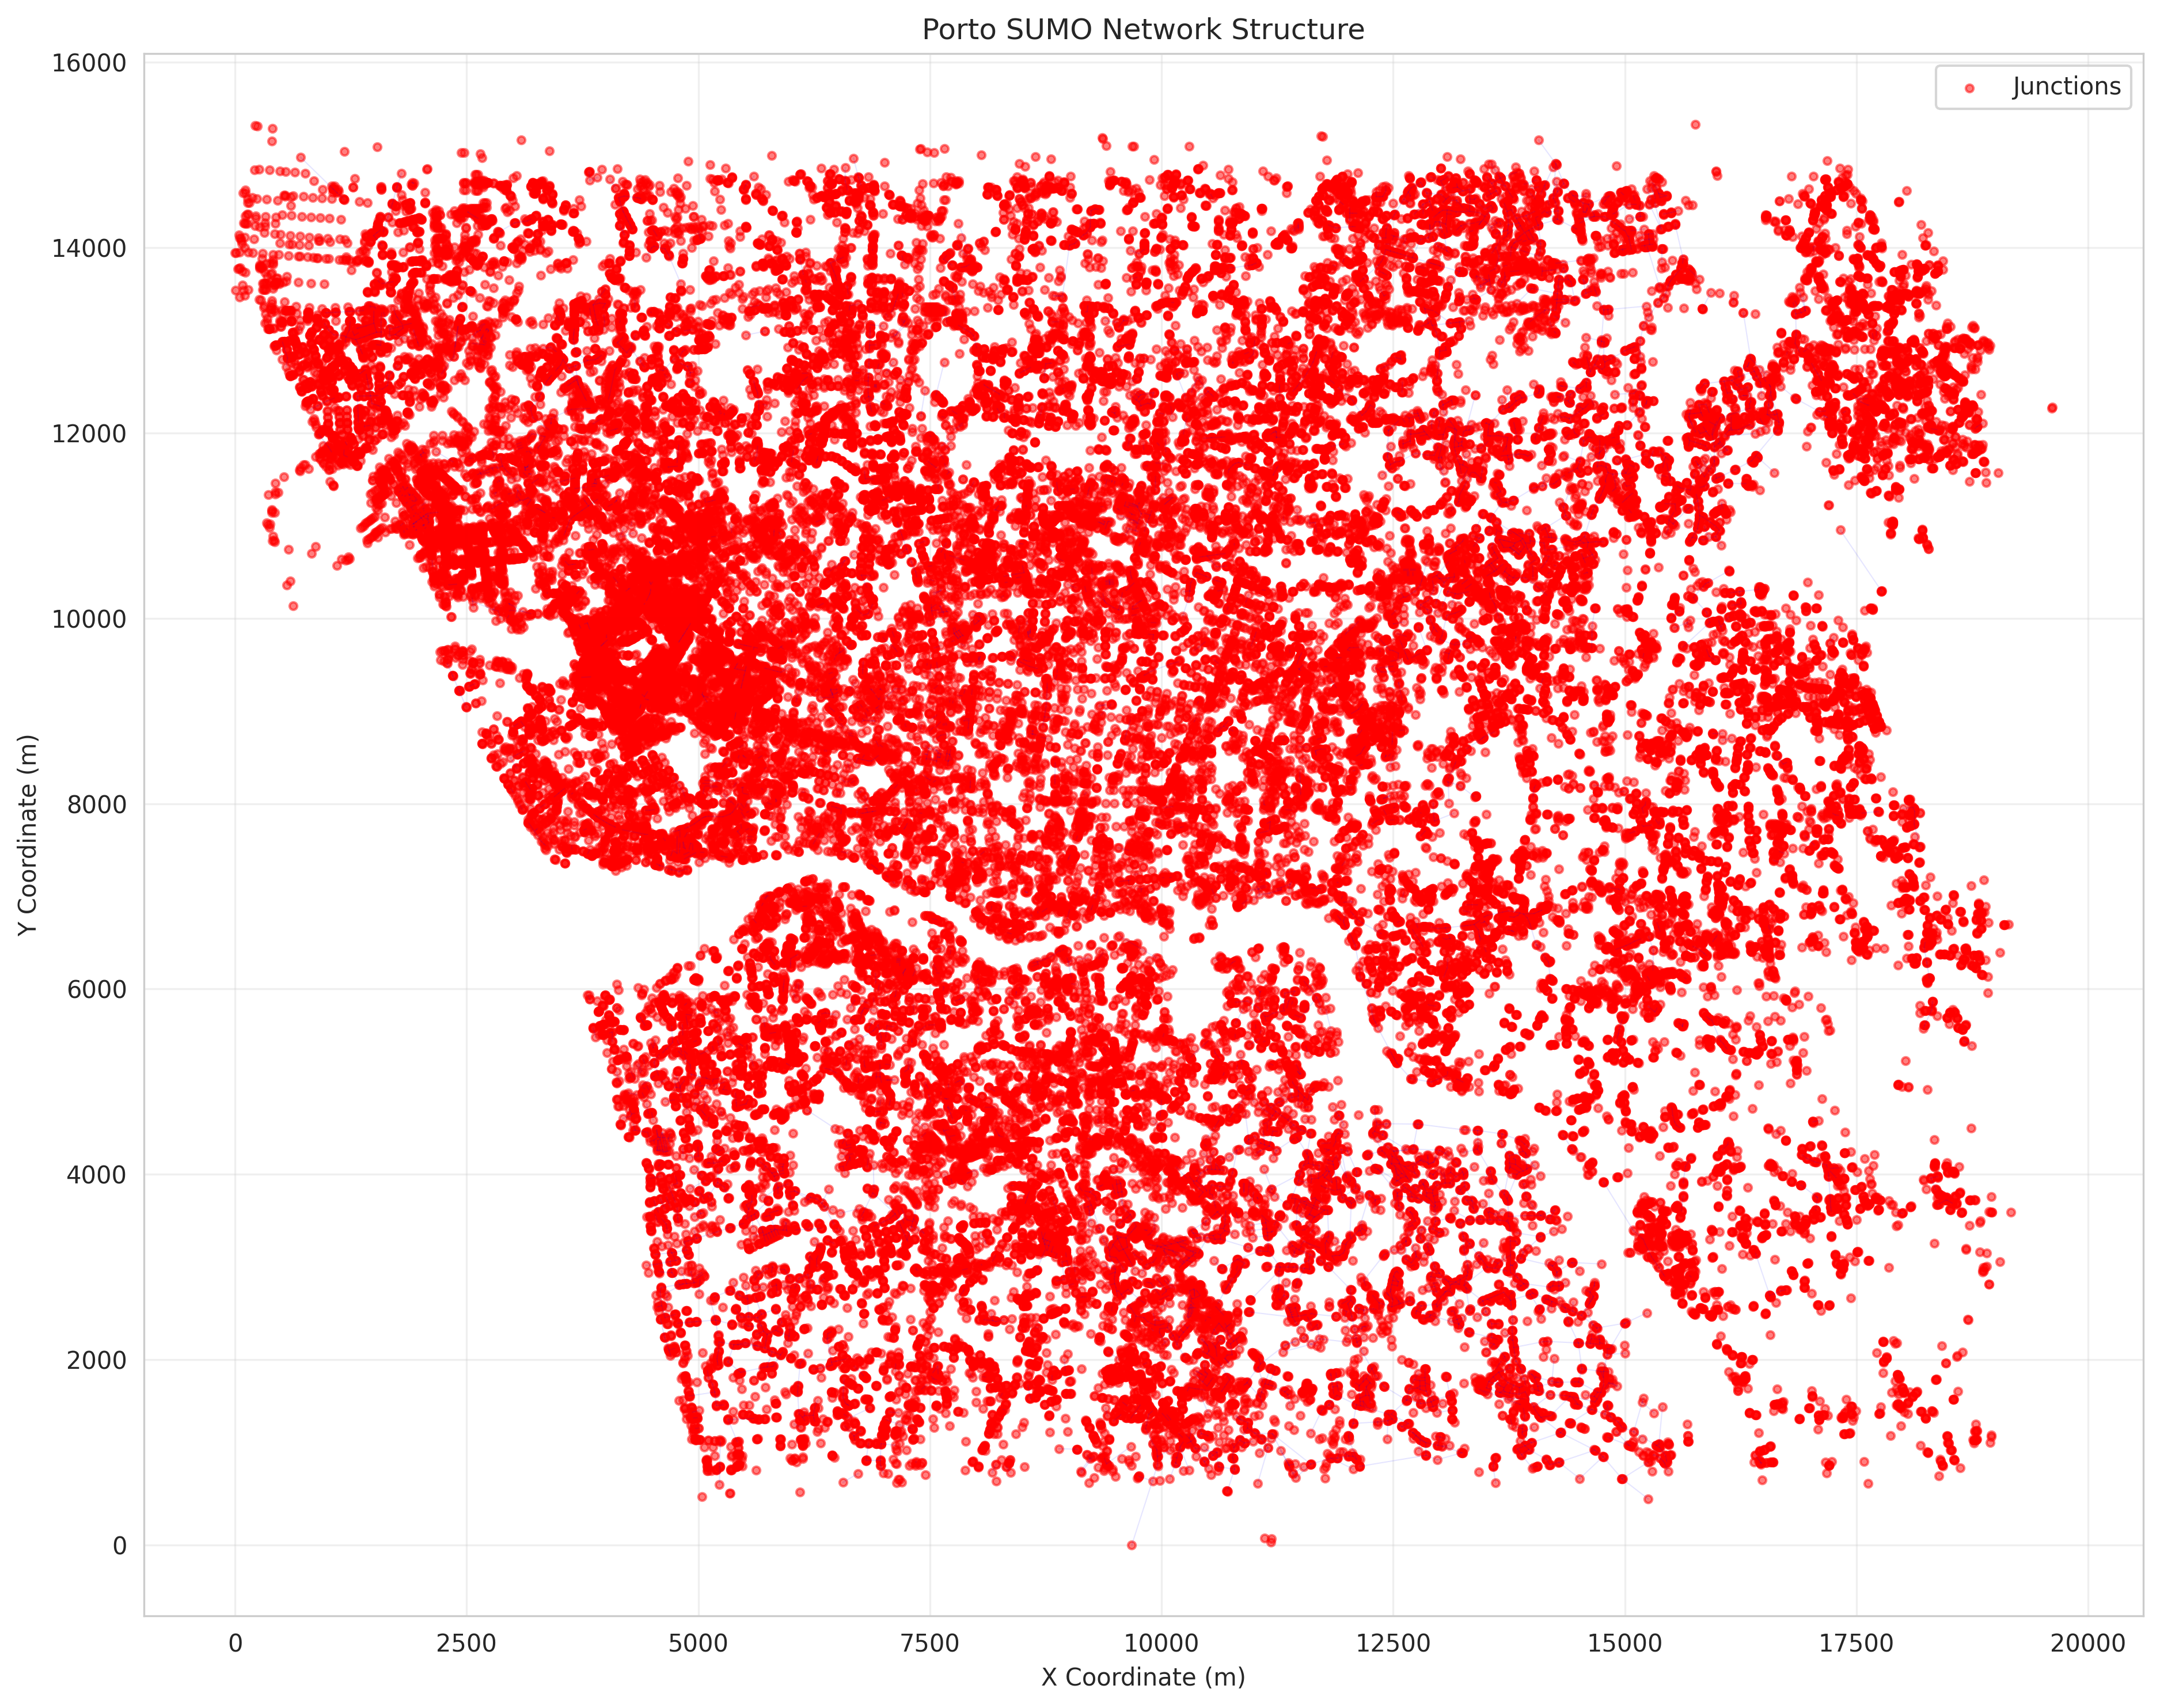
\includegraphics[width=0.9\textwidth]{figures/network_visualization.png}
\caption{Porto SUMO Network Structure}
\label{fig:network_visualization}
\end{figure}

\begin{table}[H]
\centering
\caption{Porto SUMO Network Statistics}
\label{tab:network_stats}
\begin{tabular}{l r}
\toprule
\textbf{Metric} & \textbf{Value} \\
\midrule
Total Junctions & \input{figures/network_junctions.tex} \\
Total Edges & \input{figures/network_edges.tex} \\
Total Length (km) & \input{figures/network_length.tex} \\
Average Edge Length (m) & \input{figures/network_avg_edge_length.tex} \\
Network Bounding Box & (0.32, 0.00) to (19613.86, 15329.21) \\
\bottomrule
\end{tabular}
\end{table}

\subsection{Dataset Size and Coverage}

The Porto dataset contains a substantial number of taxi trajectories. Key statistics are presented in Table~\ref{tab:dataset_stats}.

\begin{table}[H]
\centering
\caption{Porto Dataset Statistics}
\label{tab:dataset_stats}
\begin{tabular}{l r}
\toprule
\textbf{Metric} & \textbf{Value} \\
\midrule
Total Trips & 1,710,670 \\
Unique Taxis & \input{figures/dataset_unique_taxis.tex} \\
Total GPS Points & 83,409,386 \\
Average Points per Trip & \input{figures/dataset_avg_points.tex} \\
Date Range & 2013-07-01 to 2014-06-30 \\
\bottomrule
\end{tabular}
\end{table}

\subsection{Missing and Invalid Data Analysis}

Analysis of missing and invalid data reveals several quality issues:

\begin{itemize}
    \item \textbf{Missing GPS Points}: \input{figures/missing_points_pct.tex}\% of expected GPS points are missing
    \item \textbf{Invalid Coordinates}: \input{figures/invalid_coords_pct.tex}\% of GPS coordinates are outside the Porto bounding box
    \item \textbf{Large Jumps}: \input{figures/large_jumps_pct.tex}\% of trajectory segments contain jumps exceeding 1000 meters
    \item \textbf{Short Trajectories}: \input{figures/short_trajectories_pct.tex}\% of trips have fewer than 5 GPS points
\end{itemize}

Figure~\ref{fig:data_quality} visualizes the distribution of data quality issues across the dataset.

\begin{figure}[H]
\centering
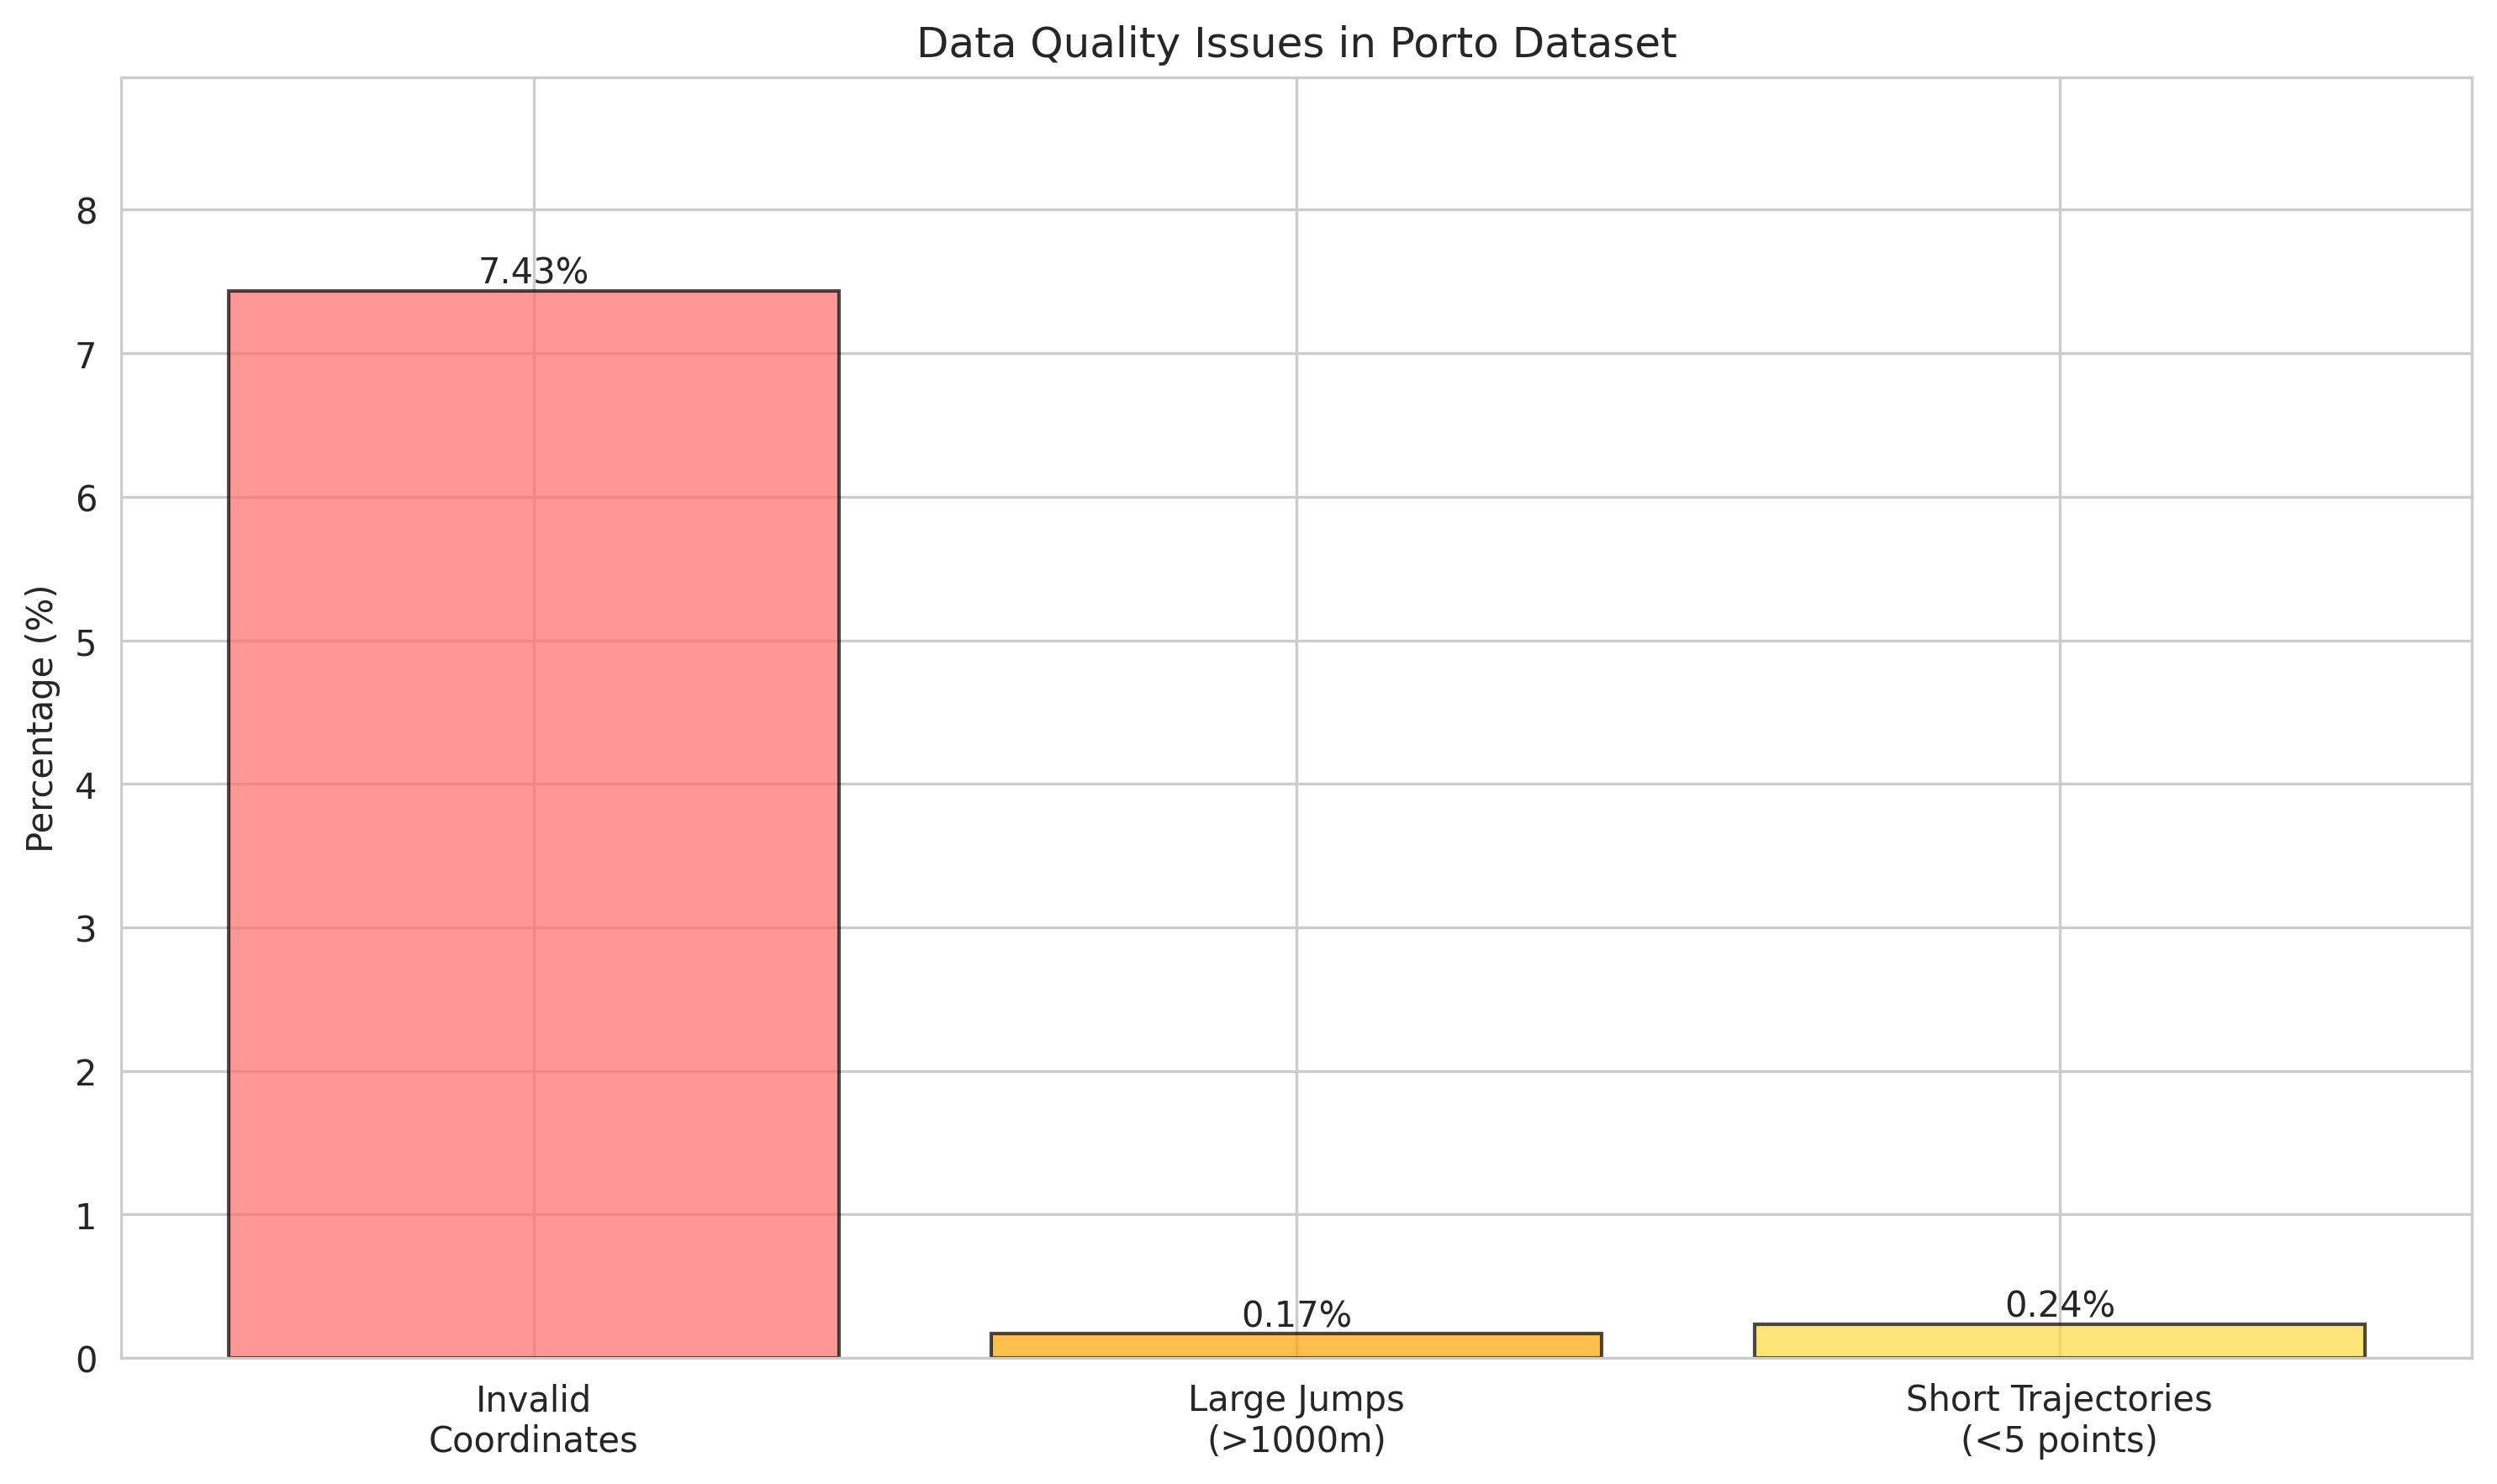
\includegraphics[width=0.7\textwidth]{figures/data_quality.png}
\caption{Summary of Data Quality Issues in Porto Dataset}
\label{fig:data_quality}
\end{figure}

\subsection{Statistical Analysis of Trajectories}

\subsubsection{Trajectory Length Distribution}

The distribution of trajectory lengths (in terms of GPS points and distance) is shown in Figure~\ref{fig:trajectory_length}. Most trajectories contain between 10 and 100 GPS points, with a median length of approximately \input{figures/median_trajectory_length.tex} points.

\begin{figure}[H]
\centering
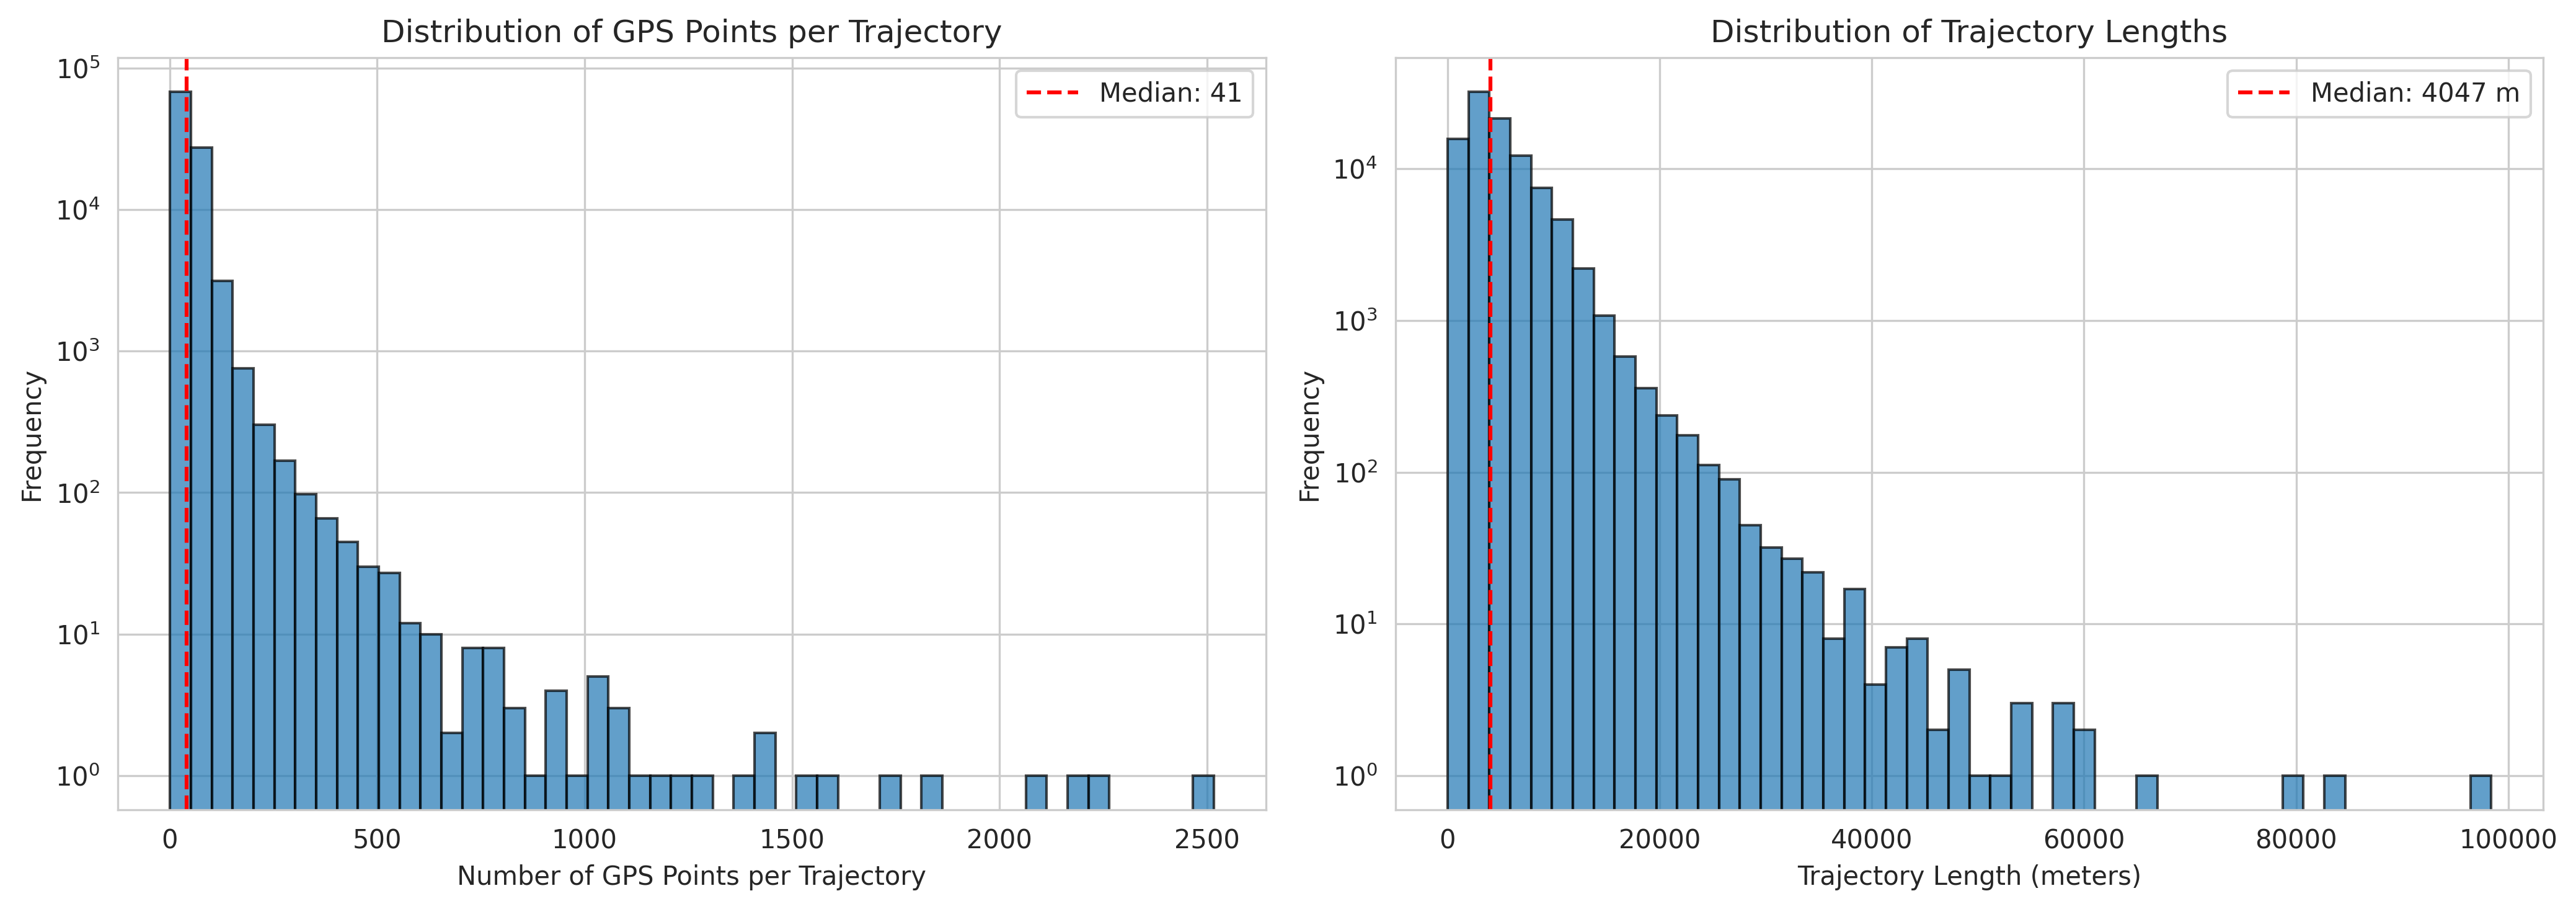
\includegraphics[width=0.9\textwidth]{figures/trajectory_length.png}
\caption{Distribution of Trajectory Lengths (GPS Points and Distance)}
\label{fig:trajectory_length}
\end{figure}

\subsubsection{Travel Time Distribution}

The distribution of travel times (calculated from timestamps) is shown in Figure~\ref{fig:travel_time}. The distribution is right-skewed, with most trips lasting between 5 and 30 minutes.

\begin{figure}[H]
\centering
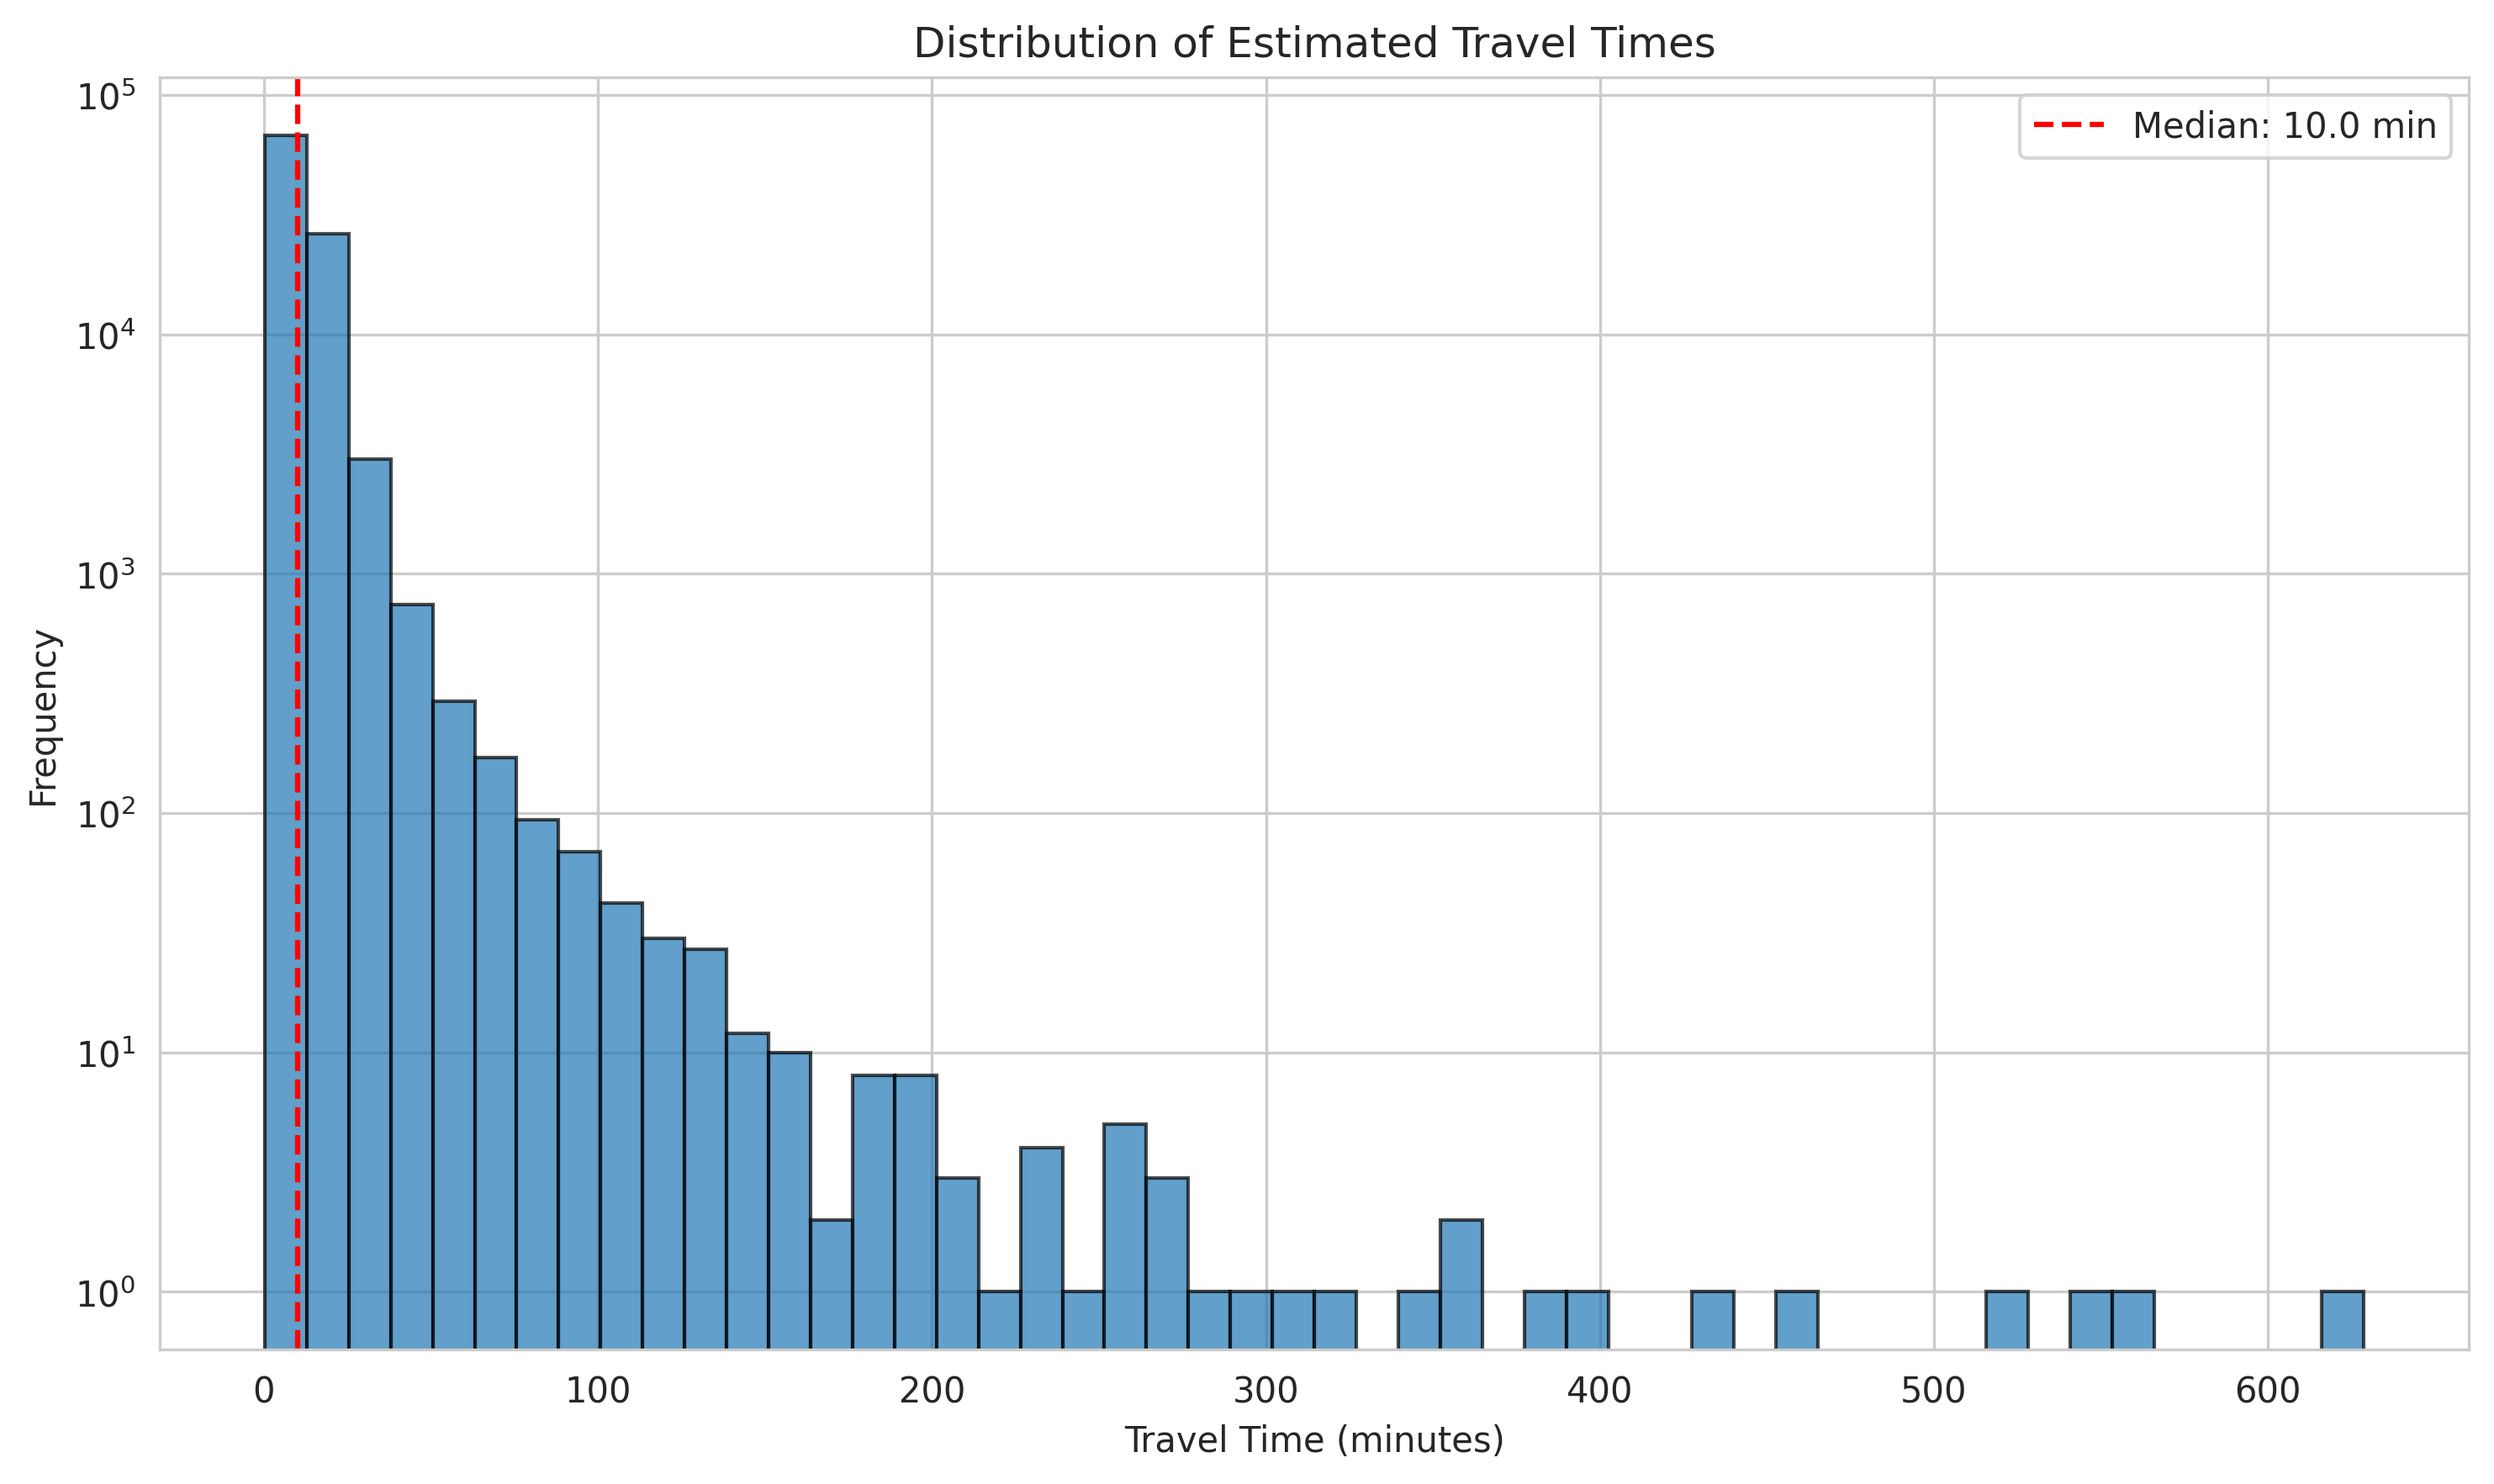
\includegraphics[width=0.7\textwidth]{figures/travel_time.png}
\caption{Distribution of Estimated Travel Times}
\label{fig:travel_time}
\end{figure}

\subsubsection{Speed Distribution}

The distribution of speeds (calculated from GPS coordinates and timestamps) is shown in Figure~\ref{fig:speed_dist}. The distribution shows typical urban driving speeds, with a peak around 30-50 km/h.

\begin{figure}[H]
\centering
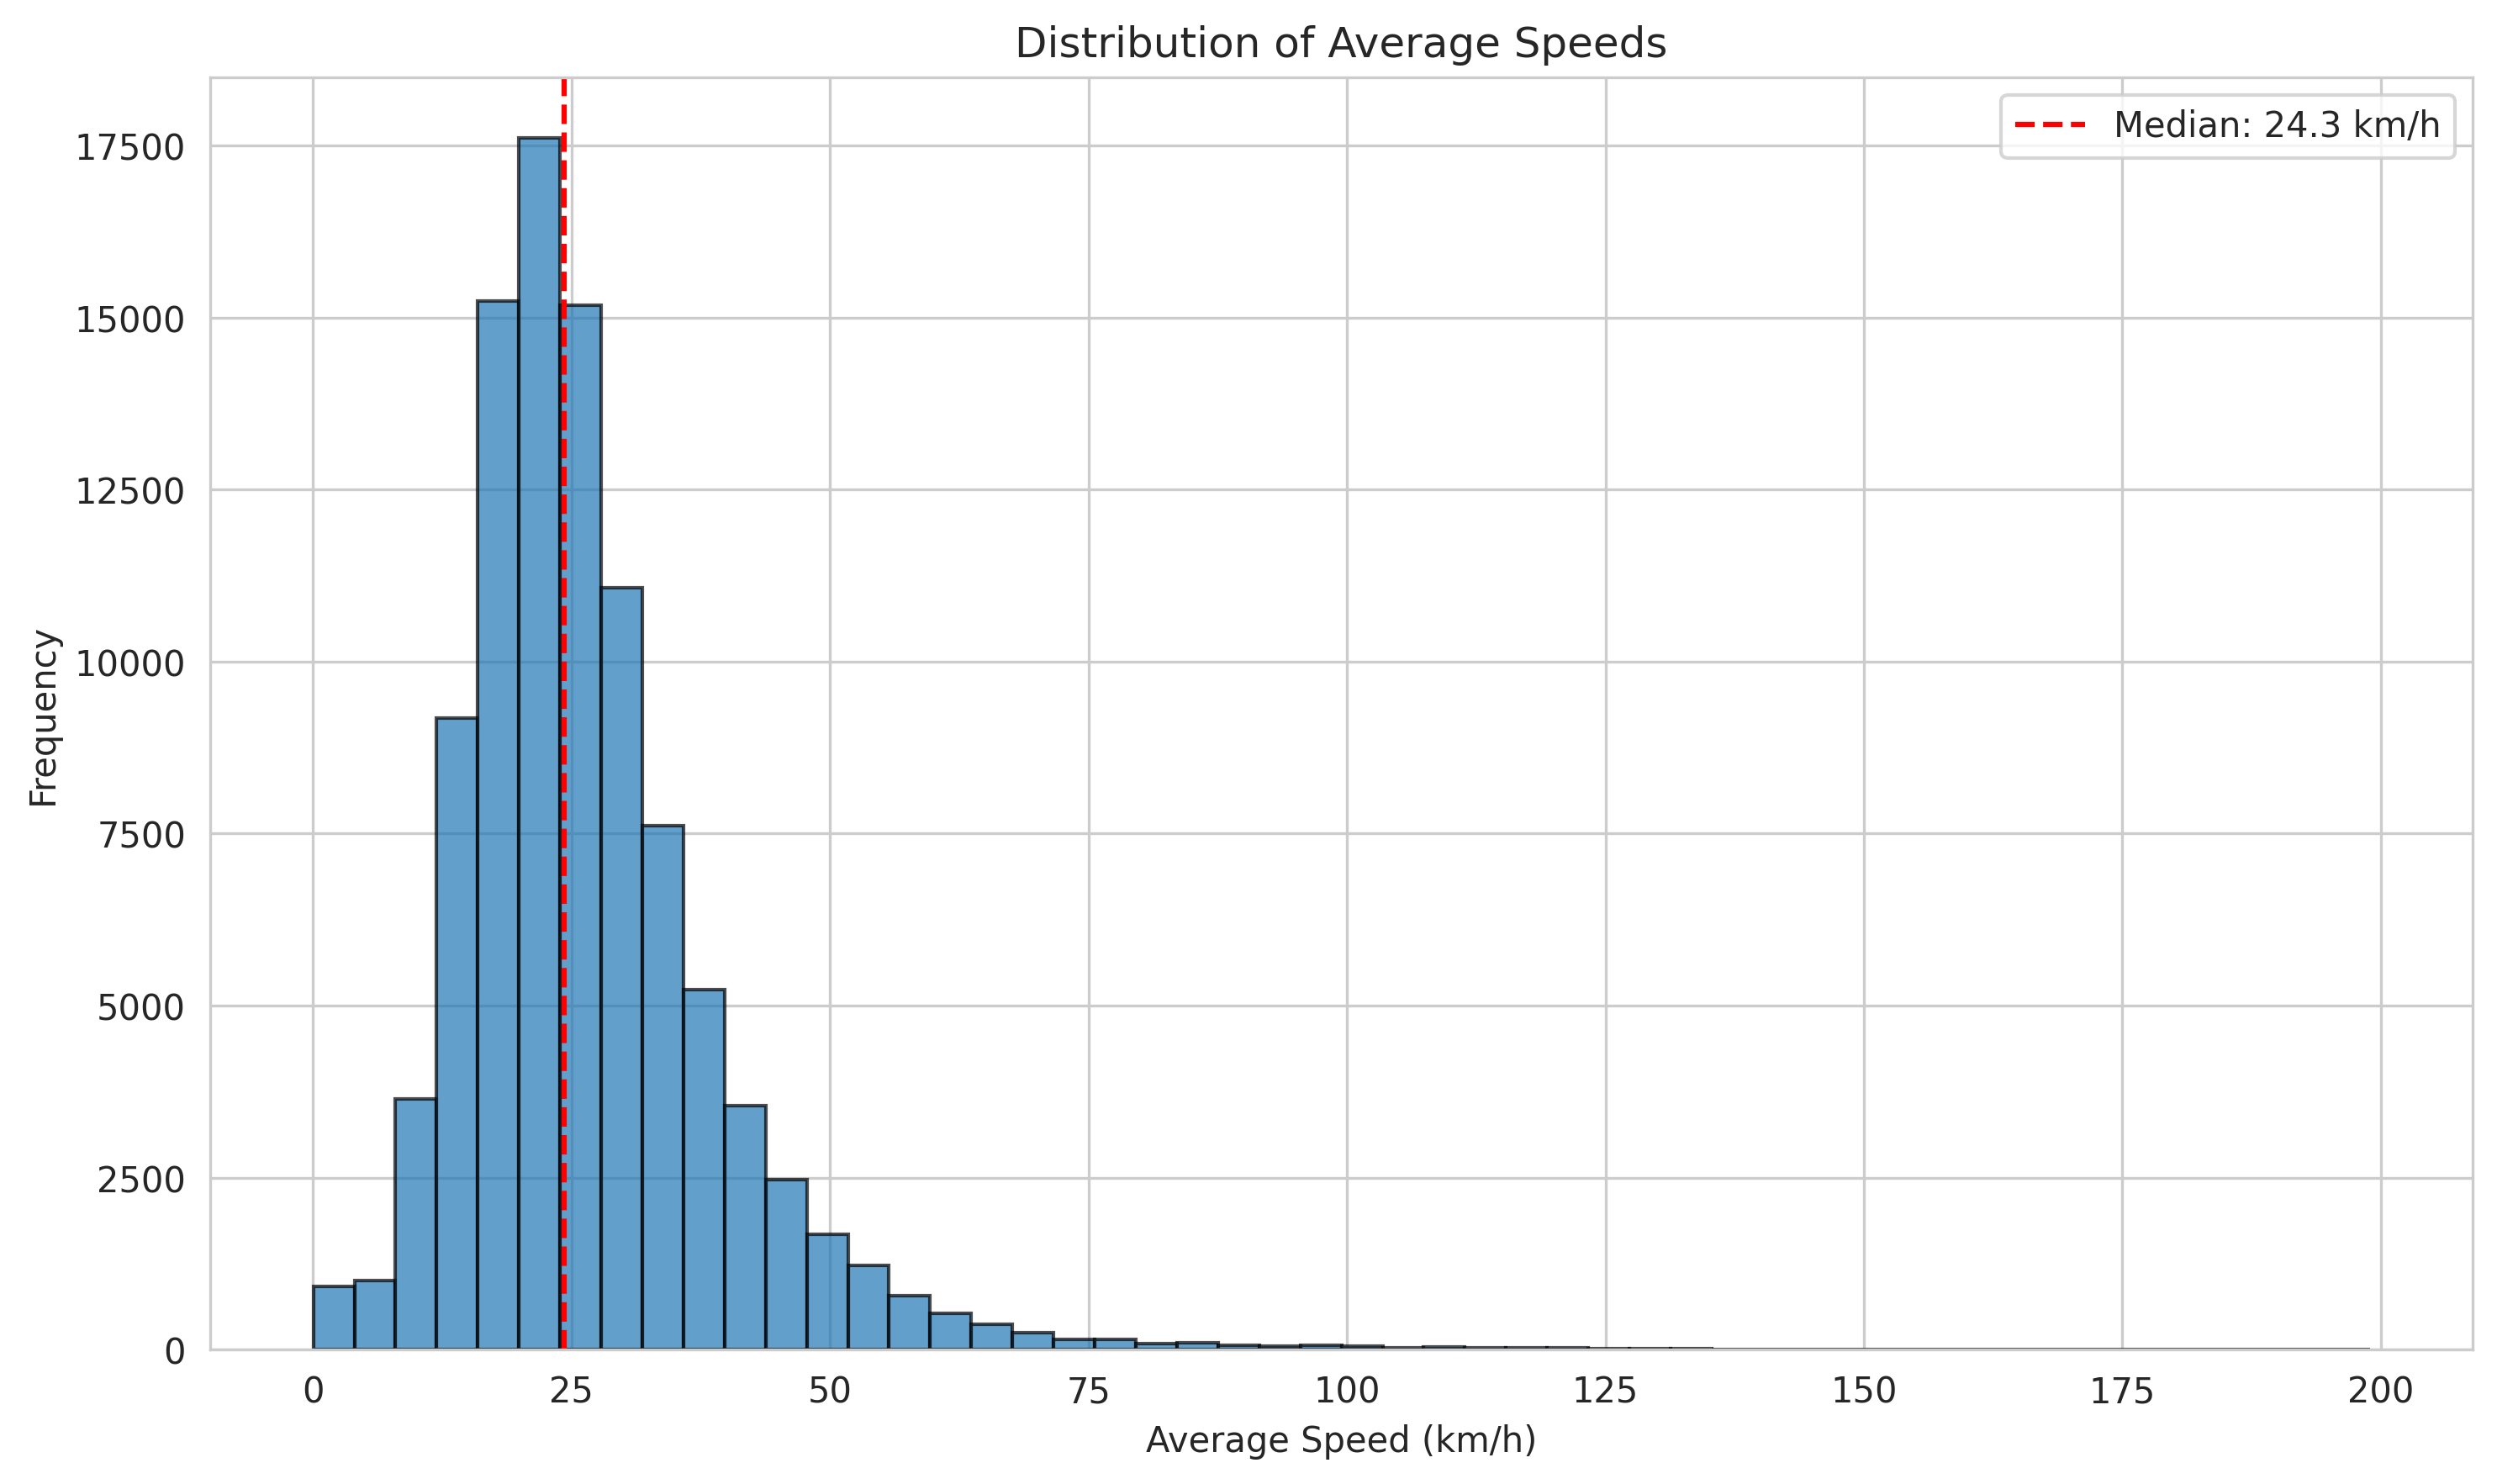
\includegraphics[width=0.7\textwidth]{figures/speed_dist.png}
\caption{Distribution of Average Speeds}
\label{fig:speed_dist}
\end{figure}

\subsubsection{GPS Jump Analysis}

The distribution of GPS coordinate jumps (distance between consecutive points) is shown in Figure~\ref{fig:gps_jumps}. The analysis reveals that while most jumps are reasonable (less than 100 meters), there are significant outliers exceeding 1000 meters that must be filtered.

\begin{figure}[H]
\centering
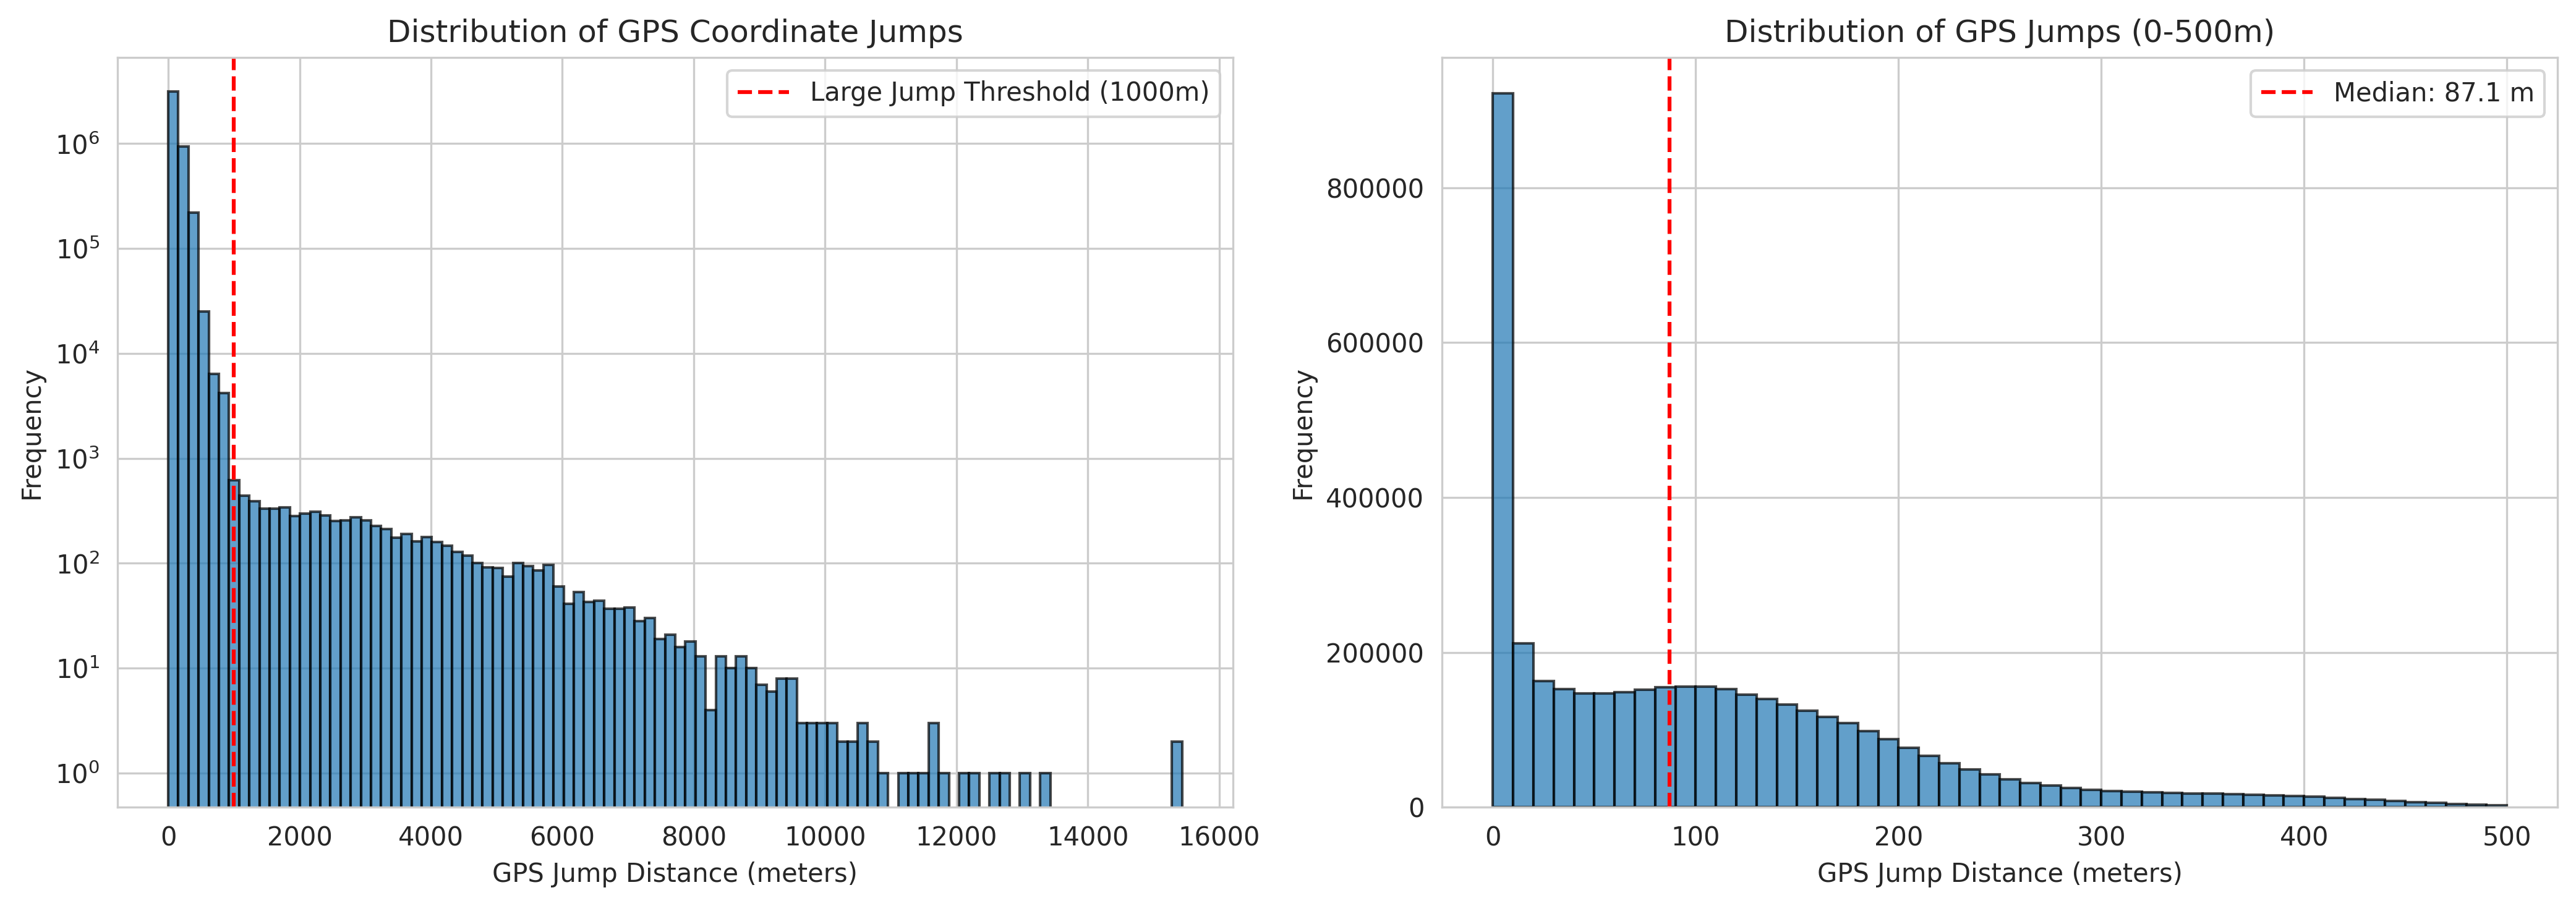
\includegraphics[width=0.9\textwidth]{figures/gps_jumps.png}
\caption{Distribution of GPS Coordinate Jumps}
\label{fig:gps_jumps}
\end{figure}

\subsubsection{Spatial Coverage}

Figure~\ref{fig:spatial_coverage} shows the spatial distribution of GPS points across Porto. The coverage is denser in central areas and sparser in peripheral regions, reflecting taxi demand patterns.

\begin{figure}[H]
\centering
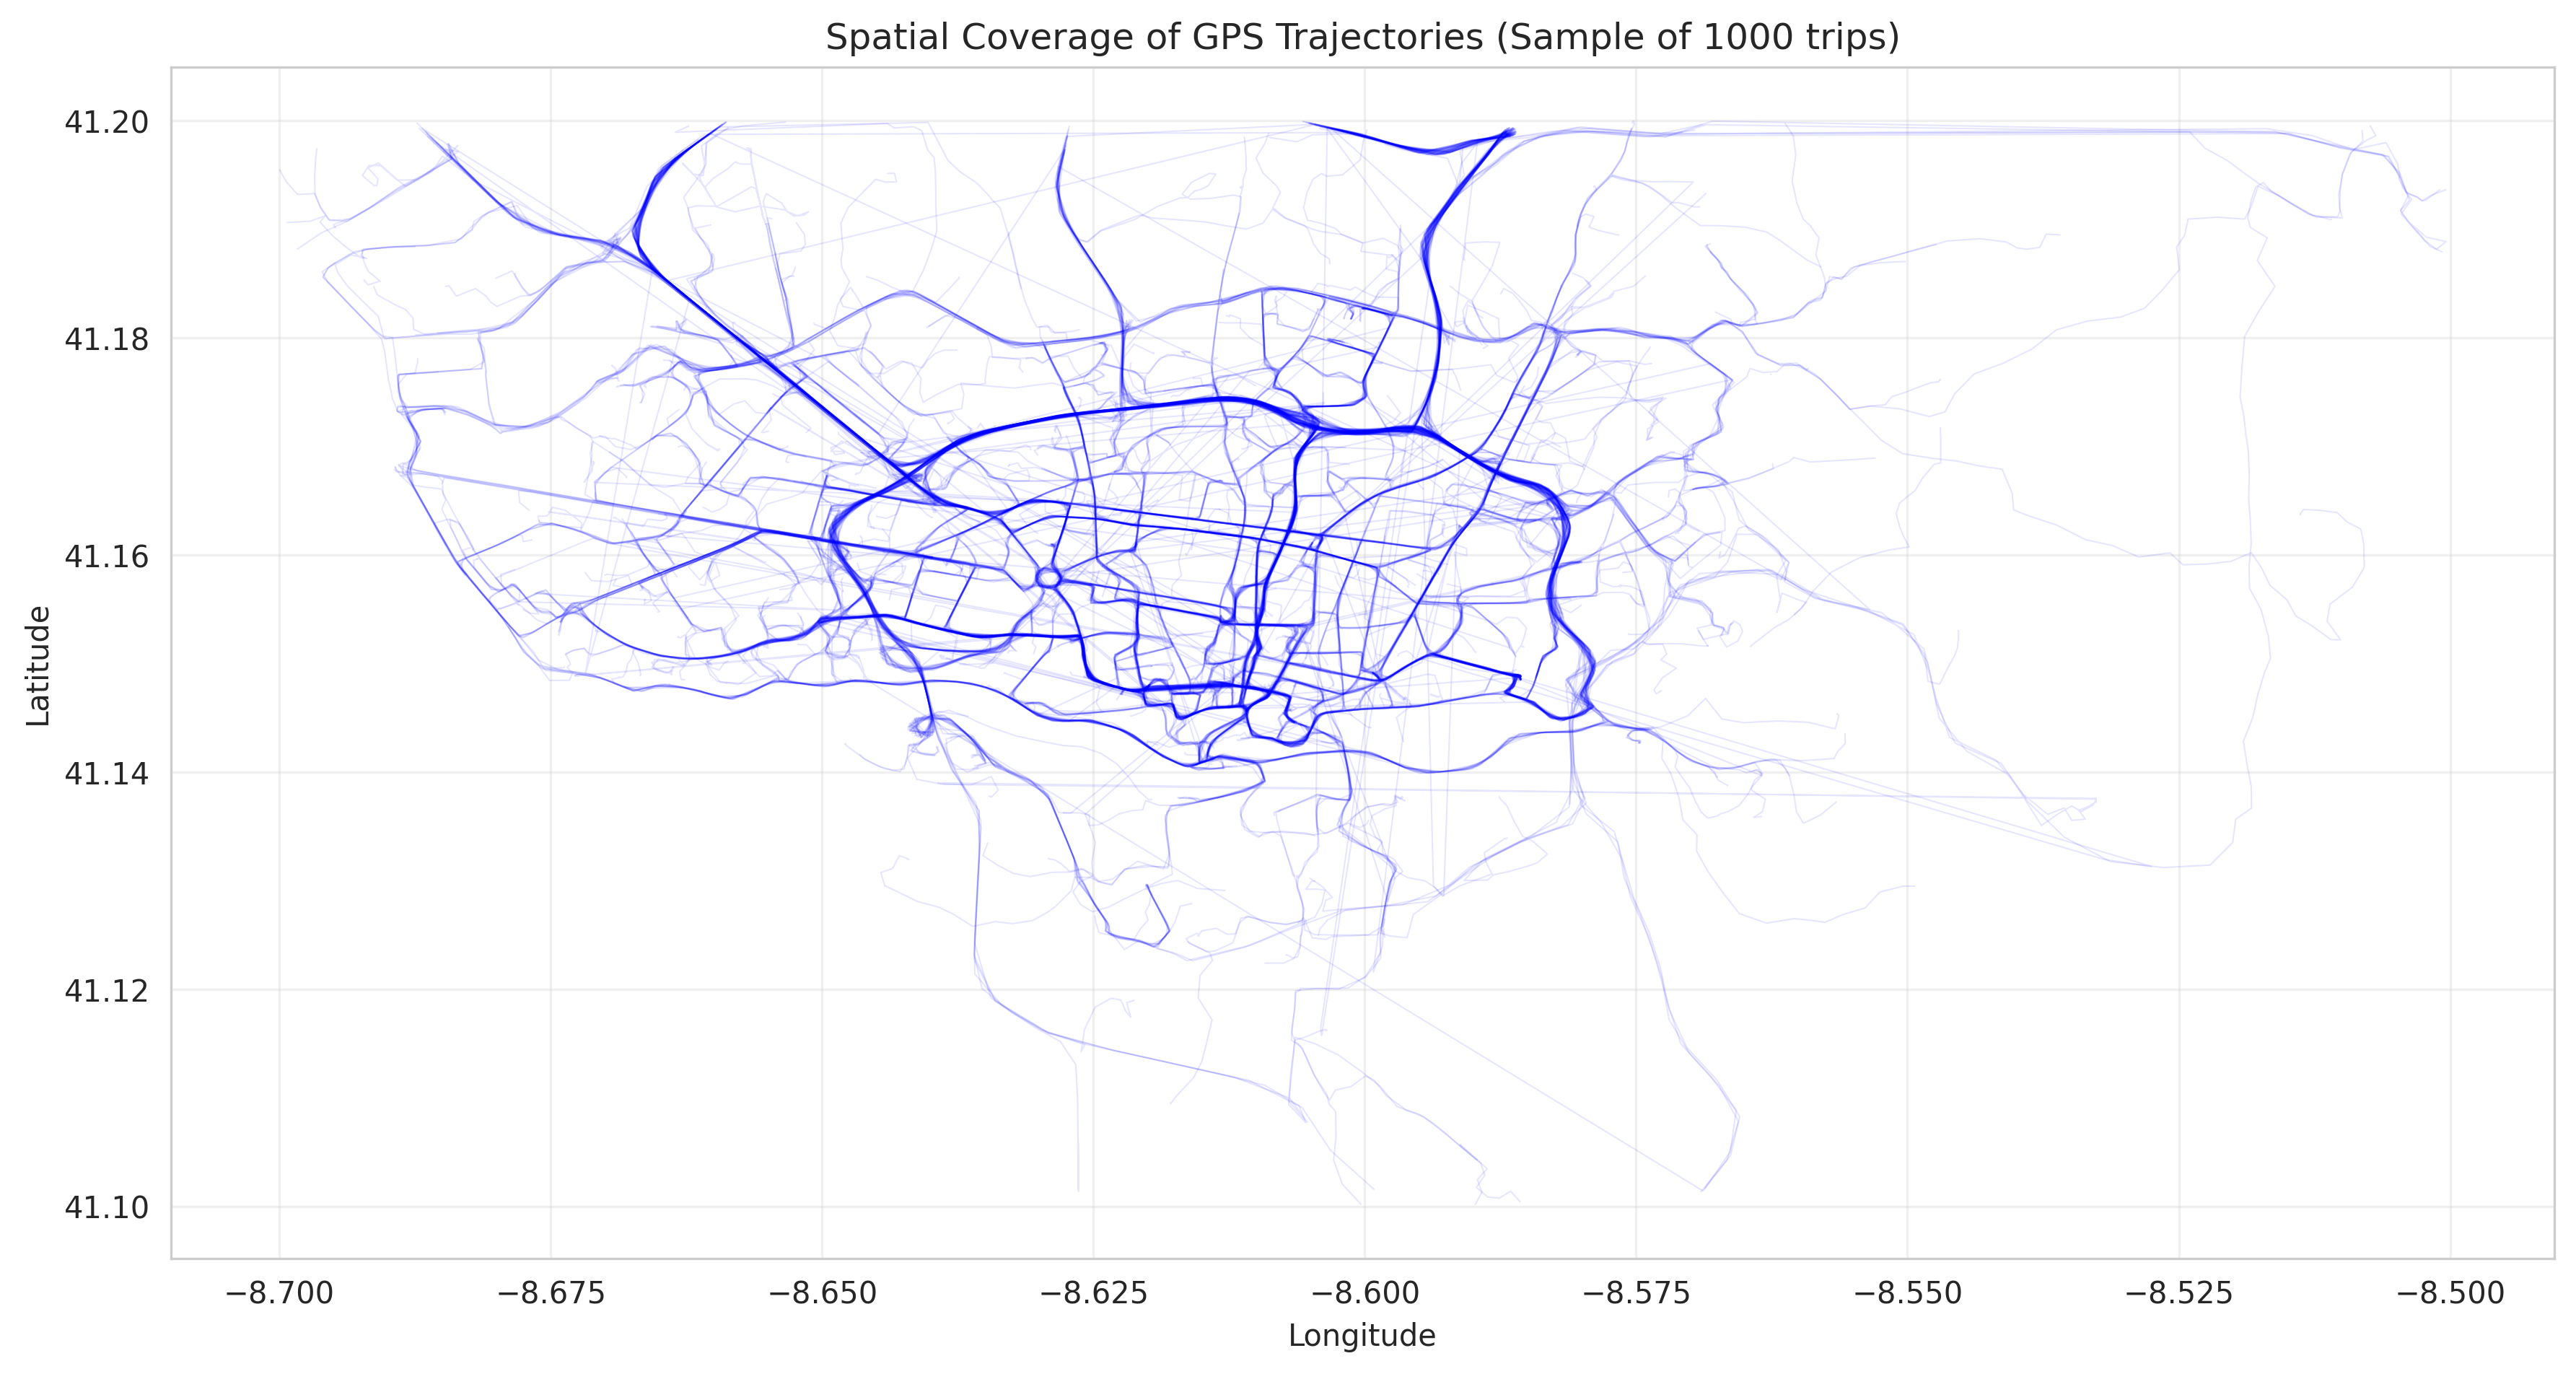
\includegraphics[width=0.8\textwidth]{figures/spatial_coverage.png}
\caption{Spatial Coverage of GPS Trajectories}
\label{fig:spatial_coverage}
\end{figure}

\section{Current Tool Status}

The Porto-to-DSTRA conversion tool is currently in a partially completed state. The following components have been implemented:

\begin{itemize}
    \item Basic CSV parsing for Porto dataset
    \item GPS trajectory extraction and parsing
    \item Initial map matching framework
    \item SUMO network loading and analysis
\end{itemize}

However, several issues remain to be addressed:

\begin{itemize}
    \item Robust handling of GPS inaccuracies and jumps
    \item Accurate identification of pickup/dropoff periods
    \item Complete map matching to SUMO edges
    \item Validation of edge sequences against SUMO network
    \item Generation of DSTRA-compatible graph snapshots
    \item Sensor-based dataset variant generation
\end{itemize}

\section{Next Steps}

The following steps are planned to complete the tool:

\begin{enumerate}
    \item Implement robust GPS jump detection and filtering
    \item Develop accurate pickup/dropoff point identification
    \item Complete map matching algorithm with SUMO network validation
    \item Generate DSTRA-compatible dynamic graph snapshots
    \item Implement sensor-based dataset variant
    \item Validate converted dataset quality and completeness
    \item Perform comprehensive testing on sample trajectories
\end{enumerate}

\section{Conclusion}

This progress report documents the current state of the Porto dataset conversion tool. While significant progress has been made, several challenges remain, particularly related to data quality issues inherent in taxi GPS trajectories. The exploratory data analysis provides valuable insights into the dataset characteristics and will guide the development of robust preprocessing and conversion algorithms.

\appendix

\section{EDA Scripts and Methodology}

The exploratory data analysis was performed using Python scripts that:
\begin{itemize}
    \item Parse the Porto CSV dataset
    \item Extract and validate GPS trajectories
    \item Analyze SUMO network structure
    \item Compute statistical distributions
    \item Generate visualizations
\end{itemize}

All scripts are available in the project repository for reproducibility.

\end{document}

